\documentclass[a4paper,12pt]{article}

\usepackage{graphicx}
\usepackage{caption}
\usepackage{subcaption}
\usepackage{tikz}
\usepackage{pgf}
\usepackage{amsmath}
\usetikzlibrary{arrows.meta}
\usepackage[utf8]{inputenc}
\usepackage[english,greek]{babel}
\usepackage{hyperref}

\title{Προσομοίωση και Μοντελοποίηση \newline Δυναμικών Συστημάτων \newline Εργασία 1}
\author{Ρουσομάνης Γεώργιος (ΑΕΜ: 10703)}
\date{Απρίλιος 2025}

\begin{document}

\maketitle

\section*{Εισαγωγή}
Σκοπός της εργασίας είναι η εκτίμηση αγνώστων παραμέτρων με χρήση της μεθόδου μέγιστης καθόδου και της 
μεθόδου σχεδίασης κατά \selectlanguage{english}Lyapunov\selectlanguage{greek} (παράλληλη και μικτή τοπολογία).
Οι μέθοδοι αυτοί ονομάζονται μέθοδοι πραγματικού χρόνου ή online γιατί δίνουν εκτίμηση μέσα σε χρόνο μιας 
δειγματοληψίας. Για την εκτίμηση αυτή, οι αλγόριθμοι πραγματικού χρόνου στηρίζονται στην τρέχουσα τιμή και 
στην αμέσως προηγούμενη, δουλεύουν δηλαδή αναδρομικά. Απευθύνονται κυρίως σε εφαρμογές στις οποίες ο αλγόριθμος
πρέπει να είναι υπολογιστικά απλός και η διαδικασία της εκτίμησης να ολοκληρωθεί πριν λάβει χώρα η επόμενη 
δειγματοληψία. Χαρακτηριστικά παραδείγματα τέτοιων εφαρμογών είναι ο προσαρμοστικός έλεγχος συστημάτων, η 
πρόβλεψη της απόκρισης συστημάτων, η ανίχνευση και αναγνώριση βλαβών σε δυναμικά συστήματα. Η εργασία 
επικεντρώνεται στην υλοποίηση των μεθόδων στο \selectlanguage{english}MATLAB\selectlanguage{greek}, την 
κατάλληλη επιλογή των παραμέτρων σύμφωνα με την λογική του \selectlanguage{english}trial and 
error\selectlanguage{greek} και την επίδραση του θορύβου στις εκτιμήσεις.

\section*{Θέμα 1}
Το σύστημα που μελετούμε είναι το σύστημα μάζας-ελατηρίου-αποσβεστήρα με εξωτερική δύναμη, η εξίσωση του
οποίου δίνεται από τη σχέση:
\begin{equation}
    m \ddot{x}(t) + b \dot{x}(t) + k x(t) = u(t),
    \label{eq:system_ODE}
\end{equation}
όπου $x(t)$ \selectlanguage{english}[m]\selectlanguage{greek} η μετατόπιση, $m>0$ η μάζα, $b>0$ ένας σταθερός 
συντελεστής απόσβεσης, $k>0$ η σταθερά του ελατηρίου, και $u(t)$ η εξωτερική δύναμη. Θεωρούμε ότι οι πραγματικές
τιμές των παραμέτρων είναι $m=1.315$, $b=0.225$ και $k=0.725$. Θεωρούμε επίσης πως οι καταστάσεις $x(t)$, 
$\dot{x}(t)$ και η είσοδος $u(t)$ είναι μετρήσιμες. Θα εξετάσουμε τις περιπτώσεις όπου $u(t) = 2.5$ και 
$u(t) = 2.5\sin t$.

Πρώτο βήμα στην ανάλυσή μας είναι η προσομοίωση της απόκρισης του συστήματος με κάποια συνάρτηση 
\selectlanguage{english}ODE solver\selectlanguage{greek} του 
\selectlanguage{english}MATLAB\selectlanguage{greek}. Η παραπάνω ΔΕ περιγράφει ένα γραμμικό και χρονικά 
αμετάβλητο σύστημα (ΓΧΑ). Συνεπώς, μπορεί να αναπαρασταθεί από τις εξισώσεις κατάστασης:
\begin{equation}
\begin{aligned}
    \dot{x}(t) = A x(t) + B u(t) \\
    y(t) = C x(t) + D u(t)
\end{aligned}
\label{eq:state_space_equations}
\end{equation}
όπου εδώ $x(t)$ είναι το διάνυσμα καταστάσεων και $y$ η έξοδος του συστήματος.

Ξεκινώντας από την (\ref{eq:system_ODE}) έχουμε:
\begin{equation}
    \ddot{x}(t) = -\frac{b}{m} \dot{x}(t) -\frac{k}{m} x(t) + \frac{1}{m} u(t).
    \label{eq:system_ODE_2}
\end{equation}
Θέτοντας $x_1 = x(t)$ και $x_2 = \dot{x}(t)$, δηλαδή $\ddot{x}(t) = \dot{x}_2$, προκύπτει:
\begin{equation}
\begin{aligned}
    &\dot{x}_1 = x_2 \\
    &\dot{x}_2 = -\frac{b}{m} x_2 -\frac{k}{m} x_1 + \frac{1}{m} u(t).
\end{aligned}
\end{equation}
Θεωρώντας ως έξοδο $y$ την μετατόπιση $x(t)$, οι εξισώσεις κατάστασης γράφονται:
\begin{equation}
\begin{aligned}
    \begin{bmatrix}
        \dot{x}_1 \\
        \dot{x}_2
    \end{bmatrix} &= 
    \begin{bmatrix}
        0 & 1 \\
        -\frac{b}{m} & -\frac{k}{m}
    \end{bmatrix} \cdot
    \begin{bmatrix}
        x_1 \\
        x_2
    \end{bmatrix} +
    \begin{bmatrix}
        0 \\
        \frac{1}{m}
    \end{bmatrix} u(t) \\
    y &= 
    \begin{bmatrix}
        1 & 0
    \end{bmatrix} \cdot
    \begin{bmatrix}
        x_1 \\
        x_2
    \end{bmatrix}
\end{aligned}
\end{equation}
Άρα οι πίνακες $A, \, B, \, C, \, D$ είναι:
\begin{equation}
    A = 
    \begin{bmatrix}
        0 & 1 \\
        -\frac{k}{m} & -\frac{b}{m}
    \end{bmatrix}, \quad B = 
    \begin{bmatrix}
        0 \\
        \frac{1}{m}
    \end{bmatrix}, \quad C = 
    \begin{bmatrix}
        1 & 0
    \end{bmatrix}, \quad D = 0
    \label{eq:state_space_matrices}
\end{equation}
Για την επιλογή της κατάλληλης συνάρτησης \selectlanguage{english}ODE solver\selectlanguage{greek} είναι
σημαντικό να προσδιορίσουμε αν το σύστημά μας είναι άκαμτο ή μη-άκαμπτο. Η συνάρτηση μεταφοράς δίνεται από
τον τύπο:
\begin{equation}
    H(s) = C(sI-A)^{-1}B + D
\end{equation}
και με αντικατάσταση των πινάκων από την (\ref{eq:state_space_matrices}) παίρνουμε
\begin{equation}
    H(s) = \frac{1}{m} \frac{1}{s^2 + \frac{b}{m}s + \frac{k}{m}}
    \label{eq:transfer_function}
\end{equation}
Η γενική μορφή της συνάρτησης μεταφοράς δευτεροβάθμιου συστήματος δίνεται από:
\begin{equation}
    H(s) = \frac{\omega_n^2}{s^2 + 2 \zeta \omega_n + \omega_n^2}
    \label{eq:transfer_function_order_2}
\end{equation}
όπου $\omega_n$ η φυσική συχνότητα του συστήματος και $\zeta$ ο συντελεστής απόσβεσης.
Συγκρίνοντας τις σχέσεις (\ref{eq:transfer_function}) και (\ref{eq:transfer_function_order_2}) παίρνουμε:
\begin{equation}
    \begin{aligned}
        &\omega_n = \sqrt{\frac{k}{m}} \\
        &\zeta = \frac{b}{2}\sqrt{\frac{1}{mk}}
    \end{aligned}
\end{equation}
και με αντικατάσταση των $m=1.315$, $b=0.225$ και $k=0.725$ βρίσκουμε ότι $\omega_n = 0.7425$, 
$ \zeta = 0.1152$. Εφόσον ισχύει $\zeta < 1$ οι πόλοι του συστήματος είναι συζυγείς μιγαδικοί με σταθερά 
χρόνου $\tau = \frac{1}{\zeta \omega_n} = 11.7$ \selectlanguage{english}sec\selectlanguage{greek}. Επειδή
οι σταθερές χρόνου του συστήματος είναι της ίδιας τάξης μεγέθους, το σύστημα χαρακτηρίζεται ως μη-άκαμπτο.
Συνεπώς, επιλέγουμε την συνάρτηση \selectlanguage{english}ode45\selectlanguage{greek} με βήμα ολοκλήρωσης 
$dt = 0.01 < 2 \tau$.

\subsection*{Μέθοδος μέγιστης καθόδου}
Για την εκτίμηση των παραμέτρων $m$, $b$ και $k$ πρέπει αρχικά να φέρουμε το σύστημά μας σε γραμμικά
παραμετροποιήσιμη μορφή. Η (\ref{eq:system_ODE}) μπορεί να εκφραστεί ως:
\begin{equation}
    \ddot{x} = 
    \begin{bmatrix}
        \frac{b}{m} & \frac{k}{m} & \frac{1}{m}
    \end{bmatrix} \cdot
    \begin{bmatrix}
        -\dot{x} & -x & u
    \end{bmatrix}^T
    \label{eq:linearly_parameterized_form}
\end{equation}
Η παραπάνω εξίσωση περιέχει το $\ddot{x}$, το οποίο δεν είναι μετρήσιμο, γεγονός που καθιστά αδύνατη την άμεση 
εκτίμηση των παραμέτρων. Για να ξεπεράσουμε αυτό το πρόβλημα, θέτουμε $\ddot{x} = s\dot{x}$ και εφαρμόζουμε 
και στα δύο μέλη το ευσταθές φίλτρο $\Lambda(s) = s^2 + \lambda_1 s + \lambda_2$. Τότε η εξίσωση 
(\ref{eq:linearly_parameterized_form}) μετασχηματίζεται ως εξής:
\begin{equation*}
    \begin{aligned}
        \frac{s^2}{\Lambda(s)}x &= 
        \begin{bmatrix}
            \frac{b}{m} & \frac{k}{m} & \frac{1}{m}
        \end{bmatrix} \cdot
        \begin{bmatrix}
            -\frac{\dot{x}}{\Lambda(s)} & -\frac{x}{\Lambda(s)} & \frac{u}{\Lambda(s)}
        \end{bmatrix}^T 
        \Rightarrow \\
        \left(1 - \frac{\lambda_1 s + \lambda_2}{\Lambda(s)}\right)x &= 
        \begin{bmatrix}
            \frac{b}{m} & \frac{k}{m} & \frac{1}{m}
        \end{bmatrix} \cdot
        \begin{bmatrix}
            -\frac{\dot{x}}{\Lambda(s)} & -\frac{x}{\Lambda(s)} & \frac{u}{\Lambda(s)}
        \end{bmatrix}^T 
        \Rightarrow \\
        x &= 
        \begin{bmatrix}
            \frac{b}{m} - \lambda_1 & \frac{k}{m} - \lambda_2 & \frac{1}{m}
        \end{bmatrix} \cdot
        \begin{bmatrix}
            -\frac{\dot{x}}{\Lambda(s)} & -\frac{x}{\Lambda(s)} & \frac{u}{\Lambda(s)}
        \end{bmatrix}^T 
    \end{aligned}
\end{equation*}
και περνώντας στο πεδίο του χρόνου:
\begin{equation}
    x(t) = \theta^{\star T}\phi(t)
    \label{eq:linearly_parameterized_form_2}
\end{equation}
όπου $\theta^{\star}$ είναι ένα άγνωστο σταθερό διάνυσμα που εμπεριέχει τις πραγματικές τιμές των παραμέτρων 
προς εκτίμηση και $\phi(t)$ το διάνυσμα οπισθοδρόμησης που είναι μετρήσιμο. Στόχος μας είναι η εύρεση μίας 
εκτίμησης $\hat{\theta}$ του $\theta^{\star}$ και έπειτα η εύρεση των εκτιμήσεων $\hat{m}$, $\hat{b}$, 
$\hat{k}$ για κάθε χρόνο $t$. Θεωρούμε το σύστημα αναγνώρισης:
\begin{equation}
    \hat{x}(t) = \hat{\theta}(t)\phi(t),
    \label{eq:identification_system}
\end{equation}
όπου η έξοδος $\hat{x}(t)$ αποτελεί εκτίμηση της εξόδου $x(t)$ του πραγματικού συστήματος 
(\ref{eq:linearly_parameterized_form_2}). Από τις (\ref{eq:linearly_parameterized_form_2}) και 
(\ref{eq:identification_system}) σχηματίζεται το σφάλμα αναγνώρισης:
\begin{equation}
    e = x - \hat{x} = x - \hat{\theta} \phi = (\theta^{\star} - \hat{\theta}) \phi
    \label{eq:identification_error}
\end{equation}
Η μέθοδος της μέγιστης καθόδου στηρίζεται για την εύρεση της αναδρομικής εκτίμησης $\hat{\theta}$ του 
$\theta^{\star}$ στην ελαχιστοποίηση ως προς $\hat{\theta}$ κατάλληλα ορισμένης συνάρτησης κόστους του $e$.
Η συνάρτηση κόστους που επιλέγουμε είναι:
\begin{equation}
    K(\hat{\theta}) = \frac{e^2}{2} = \frac{(x - \hat{\theta}\phi)^2}{2}.
    \label{eq:cost_function}
\end{equation}
Θέλουμε λοιπόν:
\begin{equation*}
    \arg \min_{\hat{\theta}} K(\hat{\theta}).
\end{equation*}
Η αναδρομική σχέση της νέας εκτίμησης $\hat{\theta}_{k+1}$ δίνεται από:
\begin{equation}
    \hat{\theta}_{k+1} = \hat{\theta}_k -\gamma \nabla K(\hat{\theta}) = 
    \hat{\theta}_k + \gamma(x - \hat{\theta}\phi)\phi = \hat{\theta}_k + \gamma e \phi,
    \quad \hat{\theta}(0) = \theta_0
    \label{eq:gradient_descend}
\end{equation}
όπου $\gamma > 0$ μία σταθερά, $\hat{\theta}(0)$ η αρχική τιμή του $\hat{\theta}$ και $\phi$, $e$ μετρήσιμα.

Στο Σχήμα~\ref{fig:identification_error} φαίνεται το σφάλμα αναγνώρισης για $u(t) = 2.5$ με $\gamma = 10^{-5}$
(αριστερά) και $u(t) = 2.5 \sin t$ με $\gamma = 10^{-3}$ (δεξιά). Η επιλογή του $\gamma$ έγινε με την μέθοδο
\selectlanguage{english}trial and error\selectlanguage{greek}. Ειδικότερα, γνωρίζουμε ότι όταν ισχύει η ΣΕΔ,
αυξάνοντας την τιμή του $\gamma$ επιταχύνουμε την σύγκλιση του $\hat{\theta}(t)$ στο $\theta^{\star}$. Πολύ
μεγάλες τιμές του $\gamma$ όμως καθιστούν την (\ref{eq:gradient_descend}) 'άκαμπτη' και επομένως δύσκολα
αριθμητικά επιλύσιμη. Συνεπώς οι τιμές του $\gamma$ επιλέχθηκαν ως οι μέγιστες δυνατές που δεν καθιστούν την
(\ref{eq:gradient_descend}) 'άκαμπτη'.

\begin{figure}[h!]
    \centering
    \begin{subfigure}{0.45\textwidth}
        \centering
        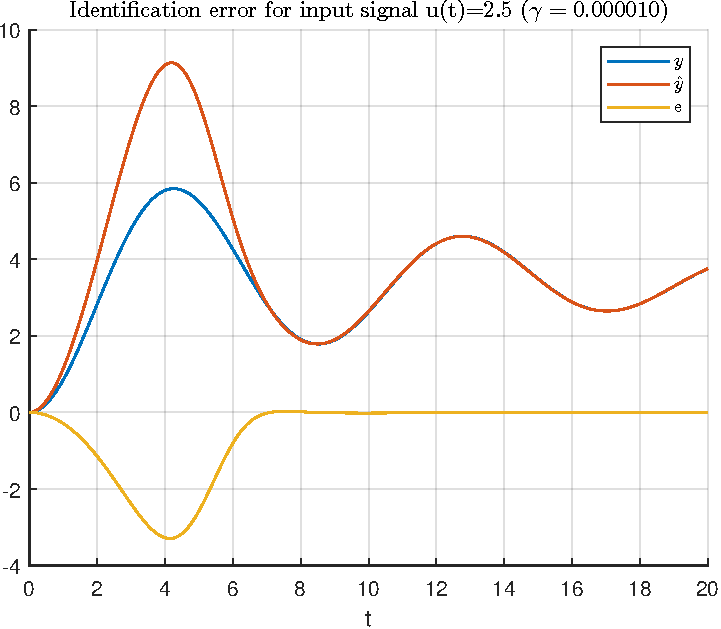
\includegraphics[width=\linewidth]{plot/identification_error_1.pdf}
        \caption{$u(t) = 2.5$}
    \end{subfigure}
    \hfill
    \begin{subfigure}{0.45\textwidth}
        \centering
        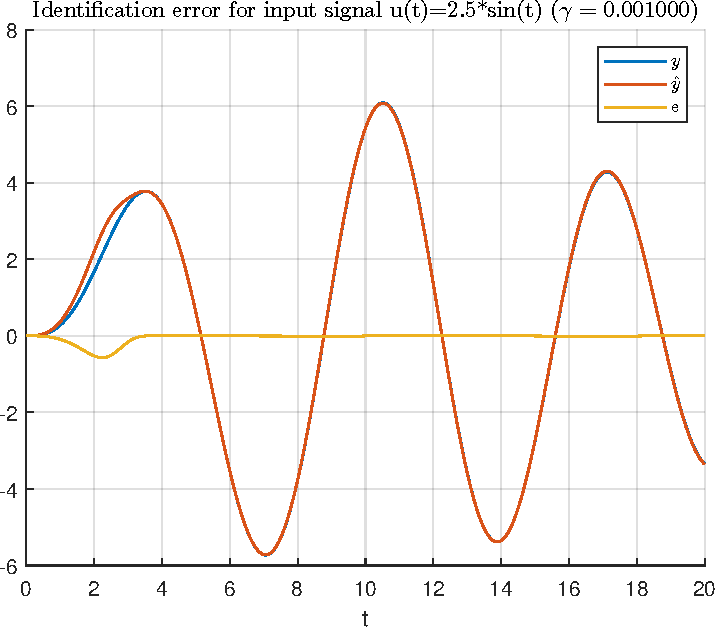
\includegraphics[width=\linewidth]{plot/identification_error_2.pdf}
        \caption{$u(t) = 2.5 \sin t$}
    \end{subfigure}
    \caption{Σφάλμα αναγνώρισης για α) $u(t) = 2.5$ και β) $u(t) = 2.5 \sin t$}
    \label{fig:identification_error}
\end{figure}


\end{document}
